\documentclass[journal]{IEEEtran}
\usepackage[a5paper, margin=10mm, onecolumn]{geometry}
\usepackage{tfrupee}
\usepackage{amsmath, amssymb, amsfonts, amsthm}
\usepackage{algorithmic}
\usepackage{graphicx}
\usepackage{textcomp}
\usepackage{xcolor}
\usepackage{txfonts}
\usepackage{listings}
\usepackage{enumitem}
\usepackage{mathtools}
\usepackage{gensymb}
\usepackage{comment}
\usepackage[breaklinks=true]{hyperref}
\usepackage{tkz-euclide} 
\usepackage{listings}
\usepackage[latin1]{inputenc}                                
\usepackage{color}                                            
\usepackage{array}                                            
\usepackage{longtable}                                       
\usepackage{calc}                                             
\usepackage{multirow}                                         
\usepackage{hhline}                                           
\usepackage{ifthen}                                           
\usepackage{lscape}
\newcommand{\myvec}[1]{\begin{pmatrix} #1 \end{pmatrix}}

\begin{document}

\bibliographystyle{IEEEtran}
\vspace{3cm}

\title{NCERT-9.5.16}
\author{EE24BTECH11042 - SRUJANA}
{\let\newpage\relax\maketitle}

\renewcommand{\thefigure}{\theenumi}
\renewcommand{\thetable}{\theenumi}
\setlength{\intextsep}{10pt} 

\numberwithin{equation}{enumi}
\numberwithin{figure}{enumi}
\renewcommand{\thetable}{\theenumi}

\textbf{QUESTION}:\\

A homogeneous differential equation of the form $\frac{dx}{dy}$ =H($\frac{x}{y}$) can be solved by substituting\\ 

(A) y =vx \hspace{2cm} (B) v =yx \hspace{2cm}
(C) x = vy \hspace{2cm} (D) x =v\\

\textbf{Theoretical Solution}:\\

\begin{align}
   \frac{dx}{dy} &= H(\frac{x}{y})  \\
   \frac{dx}{x} &= \frac{dy}{y} \cdot H\\
\end{align}
On integrating both sides , we get
\begin{align}
    \ln(x) &= \ln(y) \cdot H +C \\
\end{align}
Assume initial conditions as (1,1) and H as 2
\begin{align}
    \ln(1) &= \ln(1) \cdot 2 + C\\
    C = 0 \\
\end{align}
Solution is
\begin{align}
    \ln(x) &= \ln(y) \cdot 2\\
    x &= y^{2}
\end{align}

\textbf{Finite differences method}\\
The finite difference method is used to calculate the solutions of differential equations.\\

\begin{align}
     \frac{dx}{dy} &= \lim_{h \to 0}\frac{f(y+h)-f(y)}{h}\\
    x_{n+1} &= \frac{dx}{dy} \cdot h + x_{n}\\
    x_{n+1} &= \frac{x_n}{y_n} \cdot h + x_{n}\\
    y_{n+1} &= y_{n} + h
\end{align}
Substitute the initial conditions into the differential equation to find $\frac{dx}{dy}$ at those points. \\

Assume $h = 0.1$, and calculate $f(y+h)$. \\

Now, use $y+h$ and $f(y+h)$ as the new initial conditions. \\

Repeat this process until you have sufficient points to plot the graph. \\

Connect all points to obtain an approximate plot of the differential equation. \\

This is the graphical representation of both simulation and theoretical approaches of original differential equation

\begin{figure}[h!]
   \centering
   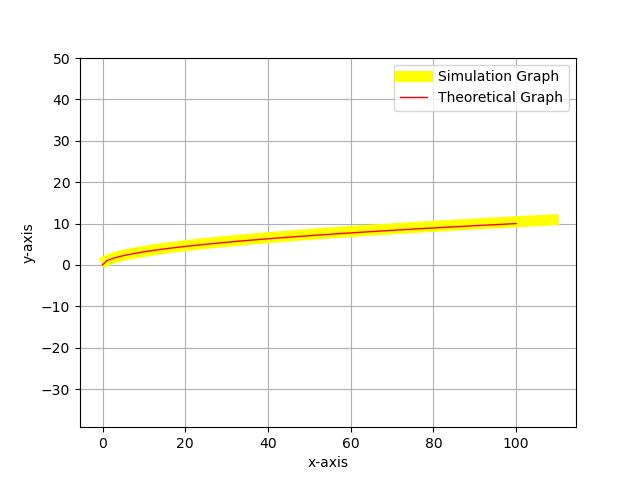
\includegraphics[width=\columnwidth]{fig/combined_fig.jpg}
\end{figure}

\end{document}

